\documentclass{article}

\usepackage{listings} % For code formatting
\usepackage[utf8]{inputenc}  % For encoding support
\usepackage{amsmath}         % For mathematical formatting
\usepackage{graphicx}        % For including images
\usepackage{xcolor}
\usepackage[a4paper, left=0.5in, right=0.5in, top=0.5in, bottom=0.5in]{geometry}  % Adjust margins here
\usepackage{tcolorbox}
\usepackage{palatino}  % Use Inconsolata font (or replace with your choice)
\usepackage{amsmath, amssymb, array, booktabs}

% Define colors
\definecolor{codebg}{RGB}{240, 240, 240}  % Light gray background
\definecolor{framecolor}{RGB}{100, 100, 100}  % Dark gray frame
\definecolor{titlebg}{RGB}{30, 30, 30}  % Dark title background
\definecolor{titlefg}{RGB}{255, 255, 255}  % White title text

% Custom lstset
\lstset{
    language=C++,                    
    basicstyle=\ttfamily\footnotesize\fontfamily{zi4}\selectfont, % Use Inconsolata
    keywordstyle=\bfseries\color{blue},        
    commentstyle=\itshape\color{gray},        
    stringstyle=\color{red},          
    numbers=left,                     
    numberstyle=\tiny\color{blue},    
    frame=single,                     
    breaklines=true,                   
    captionpos=b,                      
    backgroundcolor=\color{codebg},  % Light gray background
    rulecolor=\color{framecolor},    % Dark frame
    tabsize=4                         
}

% Custom command to add a styled heading
\newtcbox{\codebox}{colback=titlebg, colframe=titlebg, colupper=titlefg, 
  boxrule=0pt, arc=5pt, left=5pt, right=5pt, top=3pt, bottom=3pt}

\title{ByteTransformer: A High-Performance Transformer
Boosted for Variable-Length Inputs}

\author{Ayush Raina, 22148}
\date{\today}

\begin{document} 

\maketitle

\subsection*{Overview}
This paper introduces \textbf{ByteTransformer}, a high performance transformer framework optimized for \textbf{variable} length sequences. Traditional transformer architectures pad sequences to a fixed length which leads to unnecessary computations and memory utilization. ByteTransformer applies a \textbf{padding free design} that improves the efficiency by eliminating the unnecessary operations on padded tokens. The authors demonstrate that how ByteTransformer outperforms existing state of the art transformer architectures implemented across several deep learning frameworks like \textbf{PyTorch} using \textbf{Fused Multihead Attention(MHA)} which is further optimized using \textbf{CUTLASS} kernels for NVIDIA GPUs. 

\subsection*{Motivation}
Transformer models have become the foundational models in NLP tasks such as 
machine translation, language modelling etc. However modern transformer architectures like \textbf{BERT, GPT-3} have billions of parameters resulting in massive computational overhead. Existing systems apply techniques like \textbf{JIT compilations} and \textbf{graph optimizations} but all these techniques still lack support for variable length input optimizations.

\subsection*{Methodology and Key Contributions}
The authors have developed ByteTransformer, a high performance GPU accelerated transformer optimized for variable length inputs. It has been deployed for world class applications like \textbf{TikTok}. The main contributions are: \\ \\
1. \textbf{Padding Free Design: } Inputs are packed into tensors without zero padding. They calculate \textbf{positioning offset vector} for all transformer operations to maintain correct attention behaviour and keeps the whole transformer pipeline free from calculations on zero tokens. \\ \\
2. \textbf{Fused Multihead Attention Module: }They fuse MHA operations to reduce to quadratic memory and compute cost with respect to sequence length. This allowed to skip the unnecessary computations on padded tokens and improves the inference speed. This fused MHA is integrated with \textbf{NVIDIA CUTLASS} kernels. \\ \\
3. \textbf{Superior Performance: }On NVIDIA A100 GPUs, fused MHA shows upto 6.13x speedup over standard PyTorch Attention. Regarding the end to end performance, ByteTransformer surpasses PyTorch, Tensorflow, Tencent TurboTransformer, Microsoft Deep Speed and NVIDIA FastTransformer by 87\% , 131\% , 138\% , 74\% and 55\% respectively. 

\subsection*{Designs and Optimizations}
In this section we will discuss several key optimizations that ByteTransformer adopts over standard BERT encoder which involves generating the Q,K,V matrices through separate (GEMMs) which incurs significant kernel launch overhead. In ByteTransformer, these separate GEMMs are fused into a single batched GEMM operation. Additionally they pack the Q,K,V into contiguous memory to exploit locality.

\begin{figure}[h]
    \centering
    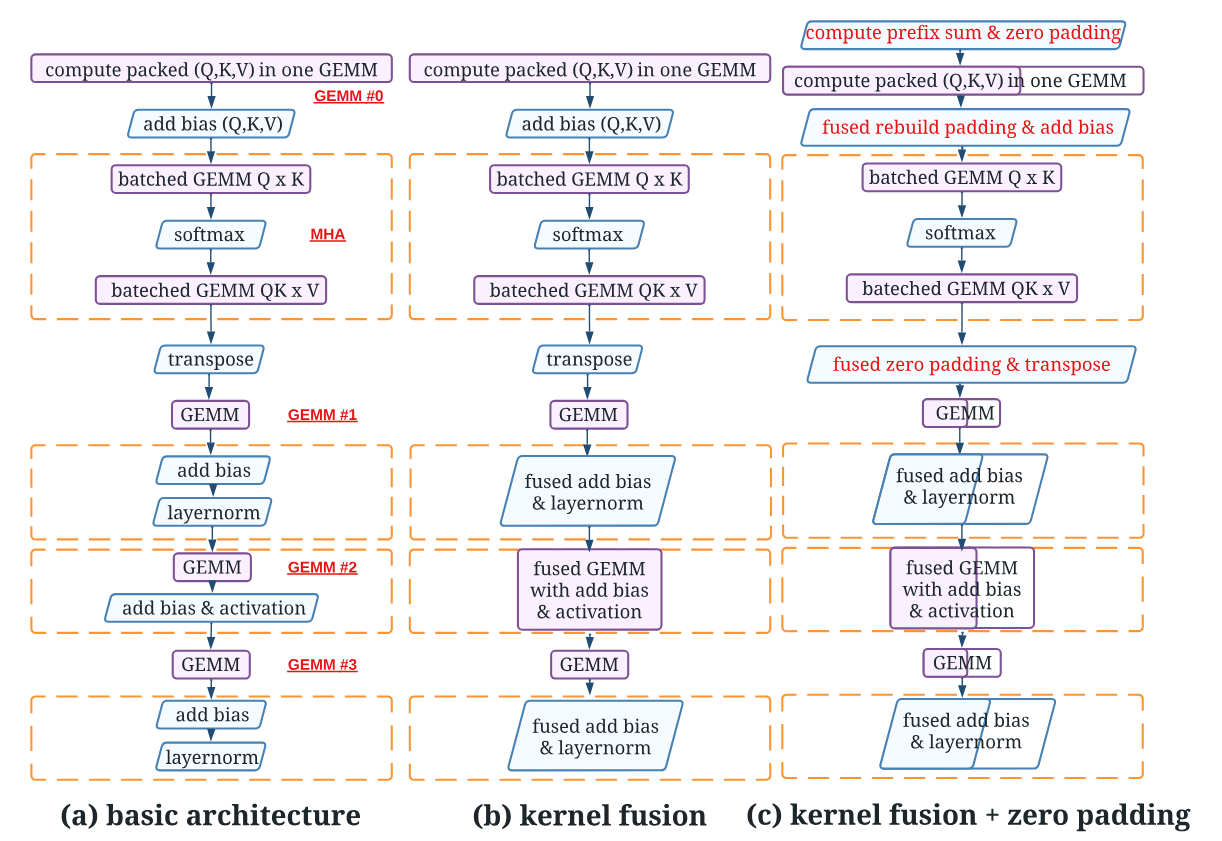
\includegraphics[width=0.3\textwidth]{architecture.png}
    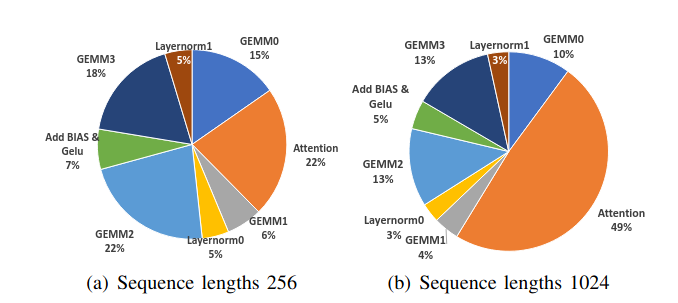
\includegraphics[width=0.5\textwidth]{performance.png}
    \caption{BERT Transformer Architecture, Optimizations and Performance for single layer}
    \label{fig:architecture}
    \vspace{-0.5cm}
\end{figure}

The authors profile a single layer BERT encoder layer (Figure 1.a) on NVIDIA A100 GPU to understand performance bottlenecks. Results show that compute bound operations like GEMMs dominate execution time at shorter sequences (61\% for L = 256) while attention operations become more dominant at longer sequences (49\% for L = 1024). Since GEMMs are already highly optimized in \textbf{cuBLAS}, the authors focus on optimizing the modules containing memory bound operations like \textbf{attention}(with softmax), \textbf{FFN}(with layernorm) and \textbf{add bias} followed by element wise activations. They optimize these operations by fusing distinct kernels and by reusing data in registers to reduce global memory accesses. Figure 1.b shows the pipeline with \textbf{add bias \& activation} fused with GEMM kernel and fused \textbf{add bias \& layernorm} kernel. \\ \\
\title{\textbf{Fused Add Bias \& Layernorm Kernel: }}After MHA, the resultant tensor needs to first be added to another tensor (bias) and perform layer normalization. The naive implementation involves 2 rounds of memory access to load and store the tensor. The Fused Kernel introduced accesses global memory only once to finish both \textbf{add bias} and \textbf{layernorm}. This fusion improved the \textbf{Single Layer BERT Transformer} performance by \textbf{3.2\%} for sequence lengths ranging from 128 to 1024 in average. \\ \\ 
\title{\textbf{Fused Add Bias \& Activation Kernel: }} After GEMM operation, the resultant tensors undergoes addition of bias and \textbf{GELU} activation. This fused implementation instead of writing the GEMM output to global memory and then reloading it, applies bias and activation directly at \textbf{register level} using a customized \textbf{CUTLASS} epilogue. Using this we further improve the performance of \textbf{Single Layer BERT Transformer} by \textbf{3.8\%} \\ \\
\title{\textbf{Optimizing for variable length inputs (zero padding algorithm): }}Instead of padding shorter sequenes with zero tokens, this algorithm packs the input tensor containing variable length sequences into a contiguous block of memory and simultaneously computes the \textbf{positioning offset vector}. This offset vector acts as an index to the original sequences during subsequent transformer operations, allowing the model to effectively skip computations on what would have been zero-padded tokens. The process involves calculating the prefix sum of a mask matrix to identify valid tokens and then using this information to pack the input tensor. This padding-free algorithm further achieved a 24.7\% acceleration of the BERT transformer when the average sequence length was 60\% of the maximum length. \\ \\ 
\title{\textbf{Optimizing Multi Head Attention: }} Even though the \textbf{zero padding algorithm} discussed above helps optimize many transformer operations like feed forward layers., it does not directly help in MHA module because batched GEMMs in MHA require uniform matrix shapes, so even if we pack our tensors in contiguous memory as discussed above, we still need to unpack and re introduce padding, bringing back inefficiency. To resolve this issue, authors propose a new \textbf{fused MHA Kernel} that works directly on contiguous packed tensors. The authors have proposed two algorithms one each for \textbf{shorter sequences} and \textbf{longer sequences}. \\ \\
\title{\textbf{Unpadded Fused Multi Head Attention for short sequences: }} For short input sequences ($L \leq 384$), they hold the \textbf{intermediate matrix} $(QK^T)$ in shared memory and registers throughout the MHA computation kernel to fully eliminate the \textbf{quadratic} memory overhead. They access the Q,K,V matrices according to positioning offset information calculated using prefix sums to avoid redundant computations on useless tokens. \\ \\
\title{\textbf{Unpadded Fused Multi Head Attention for long sequences: }} For longer input sequences ($L > 384$), the key idea is to model each MHA computation as a separate sub problem in \textbf{Grouped GEMM.} Unlike traditional batched GEMM, grouped GEMM (from NVIDIA CUTLASS) allows arbitrary shapes for each problem, making it well-suited for handling variable-length sequences.

\textbf{Fused Attention Computation: } Each MHA operation involves computing: $P_i = Q_iK_i^T, softmax(P_i), O_i = S_iV_i$. GPU Execution workflow is as follows: \textbf{CTAs (Cooperative Thread Arrays, or threadblocks)} work on different subproblems. Each CTA computes a tile (chunk of output matrix). CTAs move through subproblems in waves, until all are done. 

\textbf{Optimization 1 - Warp Prefetching: }Grouped GEMM frequently checks with the built-in scheduler on the current task assignments, which leads to the runtime overhead. In this case all 32 threads in a warp does the work together to achieve 32x fewer scheduler visit overhead.

\begin{figure}[h]
    \centering
    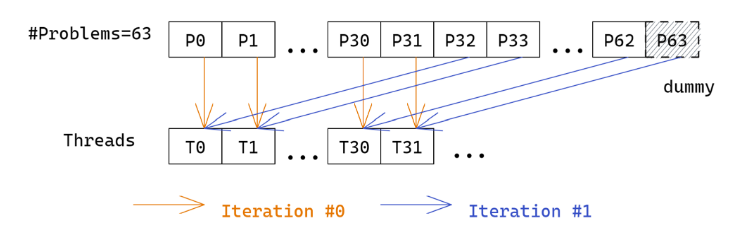
\includegraphics[width=0.5\textwidth]{prefetch.png}
    \caption{Warp Prefetching}
    \label{fig:warp_prefetching}
    \vspace{-0.5cm}
\end{figure}

\textbf{Optimization 2 - Fusing Softmax Epilogue: } After computing the first GEMM, a softmax operation is required. Instead of executing it separately, ByteTransformer fuses the softmax computation into the epilogue of first GEMM kernel. This fusion includes \textbf{intra thread reduction} followed by \textbf{intra warp reductions}. Partial results like \textbf{sum, max} are stored in global memory. Since full reduction across threadblocks is not possible within a single CTA, a lightweight auxiliary kernel completes the global reduction. However, this kernel only contributes $\sim$2\% of the total fused MHA runtime, making the epilogue fusion both efficient and practical.

\textbf{Optimization 3 - Softmax-GEMM Fusion: }To further reduce the memory traffic and hide latency, ByteTransformer fuses the element wise softmax transformation into the main loop of second GEMM, reusing the pipeline infrastructure already present in CUTLASS

\subsection*{Results}
\begin{figure}[h]
    \centering
    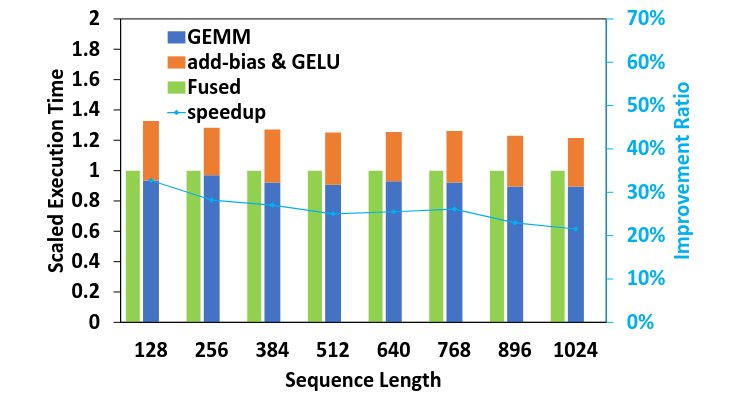
\includegraphics[width=0.4\textwidth]{addBiasAndLayerNorm.png}
    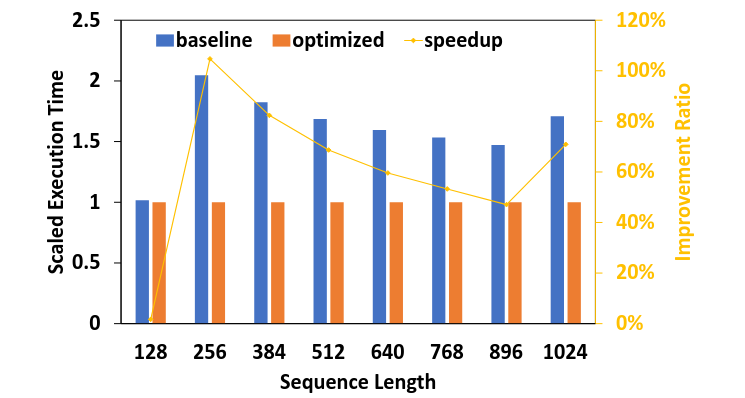
\includegraphics[width=0.4\textwidth]{addBiassGEMM.png}
    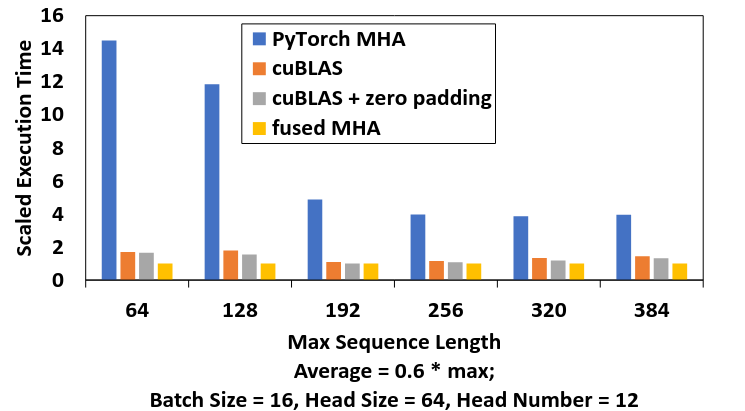
\includegraphics[width=0.4\textwidth]{mhsForShort.png}
    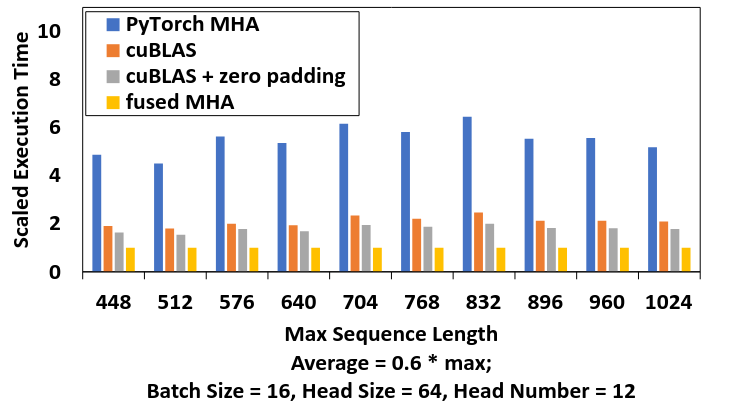
\includegraphics[width=0.4\textwidth]{mhsForLong.png}
    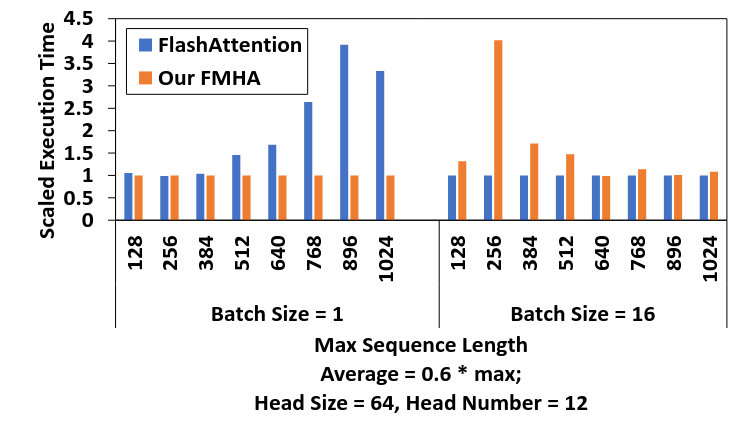
\includegraphics[width=0.4\textwidth]{compare.png}
    \label{fig:results}
    \vspace{-0.5cm}
\end{figure}
Figure 1 shows results for \textbf{Fused GEMM with Add Bias \& Activation}, Figure 2 shows results for \textbf{Fused GEMM with Add Bias \& Layernorm}, Figure 3 shows results for \textbf{Fused MHA for Short Sequences}, Figure 4 shows results for \textbf{Fused MHA for Long Sequences} and Figure 5 is for comparison with \textbf{Flash Attention}

\subsection*{Critical Analsis}
A key strength of ByteTransformer is its hardware-conscious kernel design, which effectively utilizes shared memory, cp.async pipelining, and warp-level parallelism. The proposed padding-free attention and fused softmax-GEMM kernels eliminate unnecessary memory movement and padding overhead, achieving significant real-world speedups. The warp-synchronous grouped GEMM optimization is particularly impactful, reducing scheduling overhead and boosting throughput.

However, the paper primarily evaluates kernel-level performance and does not present end-to-end model benchmarks (e.g., full finetuning or downstream accuracy). This limits visibility into the overall system impact. Also, the optimizations focus on encoder-style architectures, with limited discussion on applicability to decoders or autoregressive models.

As a potential extension, future work could focus on training-time fusion with dropout and residuals or adapting the optimizations for quantized models. This would make the approach more broadly useful for both deployment and efficient training across diverse transformer variants.
\end{document}
